\documentclass[twoside,11pt]{article}

% Any additional packages needed should be included after jmlr2e.
% Note that jmlr2e.sty includes epsfig, amssymb, natbib and graphicx,
% and defines many common macros, such as 'proof' and 'example'.
%
% It also sets the bibliographystyle to plainnat; for more information on
% natbib citation styles, see the natbib documentation, a copy of which
% is archived at http://www.jmlr.org/format/natbib.pdf

\usepackage{jmlr2e}
\usepackage{amsmath}
\usepackage{algorithm}
\usepackage{bm}
\usepackage[noend]{algpseudocode}
\usepackage{wrapfig}
\usepackage{float}

% Definitions of handy macros can go here

\newcommand{\dataset}{{\cal D}}
\newcommand{\fracpartial}[2]{\frac{\partial #1}{\partial  #2}}

% Heading arguments are {volume}{year}{pages}{submitted}{published}{author-full-names}

% \jmlrheading{1}{2017}{1-48}{4/00}{10/00}{Taylor G. Smith and Jason M. White}

% Short headings should be running head and authors last names

\ShortHeadings{Correcting Class Imbalance with Variational Autoencoders}{Smith and White}
\firstpageno{1}

\begin{document}

\title{On the Synthetic Generation of Minority Class Observations Using Variational Auto-Encoders}

\author{\name Taylor G.\ Smith \email taylor.smith@alkaline-ml.com
       \AND
       \name Jason M.\ White \email jason.m.white5@gmail.com}

\editor{Michael Bernico}
\maketitle

\begin{abstract}%   <- trailing '%' for backward compatibility of .sty file
This document describes a methodology by which to remedy imbalanced datasets for the purpose of classification. A dataset may be considered imbalanced if its classification labels are disproportionately represented across classes. In many real-world domains, class imbalance---or the presence of extremely rare events which may be costly to misclassify---is quite prevalent. Commonly cited problem domains include fraud detection, medical imaging, anomaly detection and countless more.  Our procedure furthers the Synthetic Minority Over-samping Technique \citep*{chawla2002smote}---or SMOTE---by training generative variational auto-encoders on the minority class(es) for the purpose of creating synthetic examples.
\end{abstract}

\begin{keywords}
  classification, class-imbalance, cost-sensitive learning, SMOTE, variational auto-encoders, skewed distributions
\end{keywords}

\section{Introduction}

A dataset may be considered imbalanced if its classification labels are disproportionately represented across classes. While class imbalance manifests itself in varying degrees, often times one class---the majority class---is highly represented, while one or more minority classes are present at a much smaller ratio. This paper focuses on inducing classifiers given a training set, $X \in \mathbb{R}^{m \times n}$, with a corresponding set of class labels, $y \in \{0, 1, ..., c\}$ in which one or more of the \emph{minority} class labels is/are represented at a significantly smaller proportion than that of one or more \emph{majority class} labels.

As noted by countless studies, classifier efficacy cannot meaningfully be expressed or assessed via conventional, cost-insensitive metrics such as average \emph{accuracy} (or the percentage of testing observations properly identified by the learner). This greatly complicates the classification task since such metrics will offer misleadingly optimistic scores on an otherwise poor classifier. Consider a study by \cite{lewis1994heterogeneous} in which only 0.2\% of the training samples are positive; even the worst of learning algorithms can effortlessly attain 99.8\% accuracy by simply always predicting the majority class.

One of the notable risks of working with imbalanced datasets is the seeming compounding effect they have on a modeling pipeline; model selection tasks such as grid searches can be especially confounded by this issue, since the metric a grid search is intended to optimize may lie in direct discord with the underlying cost sensitivity of the imbalanced classification task itself. While class imbalance is a common challenge in many applied machine learning domains, what makes it an particularly interesting and relevant problem is the frequent tangible cost with which misclassification of rare events is typically associated. The real-world impact of such errors can be especially perilous in the medical domain, where diagnostic datasets are especially susceptible to class disparity, as high risk examples tend to constitute the minority class \citep{rahman2013addressing}.

The machine learning community has attempted to address the problem of class imbalance in several ways: weighting---such as the development of cost-sensitive classification metrics like the ROC convex hull \citep{provost2001robust} or the F-measure \citep{lewis1994training}---and data preparation tasks that either resample or manipulate the input data before building a model. Our approach can be considered one of the latter, and seeks to synthetically augment the training set irrespective of the selected scoring metric.

Section 2 presents previous work to which our approach may be compared. Section 3 introduces generative models, and more specifically, variational auto-encoders. Section 4 outlines the details of our technique. Section 5 details the performance of our technique compared with other common class imbalance solutions. \\

\section{Previous Work}
\subsection{Over-sampling minority class samples}

Research on the efficacy of resampling as a preprocessing technique for imbalanced datasets has been extensively conducted. One common approach for resampling a training set is over-sampling the minority class examples with replacement \citep{japkowicz2000class}. She proposed several variants of over-sampling, with varying degrees of success. Her random resampling approach drew minority samples with replacement until the minority class was represented at the same magnitude as the majority class. She also proposed ``focused resampling," which only drew minority samples from along the decision boundary between the majority and minority classes. 

Of note is the fact that she observed no clear advantage between generalized over-sampling and her ``focused" over-sampling \citep{japkowicz2000class}. Using a decision tree classifier, \citet{chawla2002smote} showed that duplicating minority observations actually further narrowed the (theoretically, already very small) decision region, causing more splits in the tree and leading to overfitting.


\subsection{Under-sampling majority class samples}

In conjunction with her research on over-sampling methods, \citet*{japkowicz2000learning} showed that under-sampling the majority class can be effective---especially in tasks where $c > 2$---presenting the added benefit of reducing the training set size, and consequently the complexity of the training task. (CITE SOMETHING THAT SHOWS THE REDUCTION IN TRAINING DATA CAN BE BAD, THOUGH)

\citet*{kubat1997addressing} proposed a more sophisticated form of under-sampling by which the majority class samples are segmented into one of four categories: those suffering \emph{class-label noise}, unreliable \emph{borderline} samples that sit near the decision surface, \emph{redundant} examples, and \emph{safe} examples (archetypal to the majority class representation, and necessary for training). They showed that the noisy and border-point majority class examples could easily be recognized in the training set by identifying and removing majority class samples that form \emph{Tomek links} \citep{tomek1976two} with minority class samples.

\subsection{Synthesizing minority class samples}

Rather than simply sampling the minority class with replacement, \cite{chawla2002smote} proposed the over-sampling of synthetic minority class observations.  As previously mentioned, they implemented the SMOTE algorithm which uses randomly sampled minority class observations' \emph{k}-nearest neighbors to generalize minority class decision region neighborhoods: for each of $p$ randomly sampled minority observations, $\mathbf{x}^{(i)} \in \mathbb{R}^{n}$, compute the \emph{k}-nearest neighbors to $\mathbf{x}^{(i)}$, denoted as $\mathbf{J} \in \mathbb{R}^{k \times n}$, and generate a synthetic example between $\mathbf{x}^{(i)}$ and each nearest neighbor, $\mathbf{j}^{(l)}$:
\[
    \mathbf{x}^{(i)\prime} = \mathbf{x}^{(i)} + gap * (\mathbf{j}^{(l)} - \mathbf{x}^{(i)})
\]
where $gap$ is a random scalar between 0 and 1. The application of SMOTE has been shown to effectively aid in generalizing the decision region for the minority class(es) by synthetically generating minority class observations \citep*{chawla2002smote}. However, one of the trade-offs it makes the risk of ``\emph{over}-generalized'' minority decision regions in cases of significant class overlap.

Figure 1 shows an unbalanced dataset with significant overlap between classes. The decision regions for the minority class are narrow with respect to the total decision space, and classification performance is poor. Figure 2 shows the same dataset after being balanced by SMOTE. The decision region for the minority class, though significantly generalized, has bled so far into the majority class space as to diminish the usefulness of the classifier.

%\newpage
%\centerline{
%  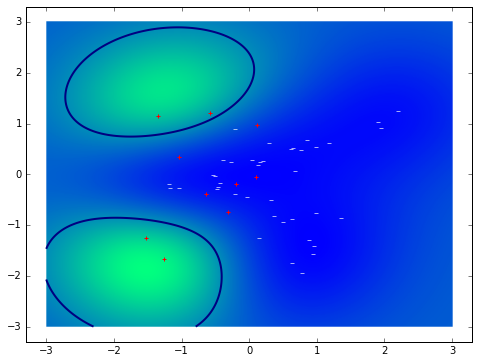
\includegraphics[scale=.6]{no-balance.png}
%}

%\newpage
\begin{figure}[H]
    \centering
    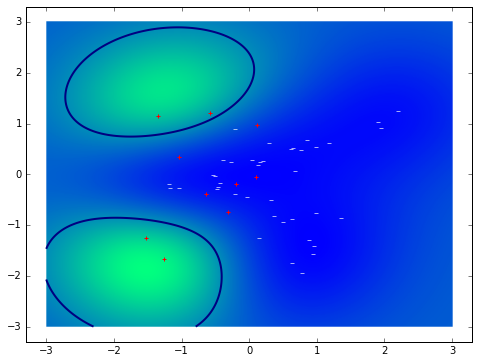
\includegraphics[scale=.5]{no-balance.png}
    \caption[width=40mm]{An SVM classifier exhibits poor performance on a highly unbalanced dataset with significant class overlap \& a narrow decision region for the positive class.}
    \label{fig:label}
\end{figure}
\begin{figure}[H]
    \centering
    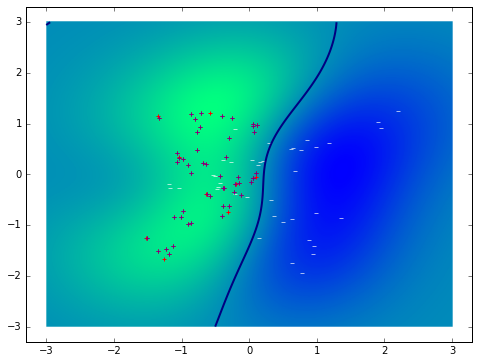
\includegraphics[scale=.5]{smote-balance.png}
    \caption[width=40mm]{The same dataset, after being balanced with SMOTE. The decision region has been over-generalized to the point of diminishing the usefulness of the classifier.}
    \label{fig:label}
\end{figure}



\section{Variational Auto-Encoders}

Generative methods are a family of unsupervised learning techniques that can be used to generate observations given some latent distribution. The advent of generative algorithms is that they do not simply learn the classification boundaries between classes, as do discriminative algorithms, but model the (often intractable) distribution by which the data was generated. As a result, generative models allow us to create new, synthetic examples by inferring the posterior. 

An auto-encoder, as originally introduced by Hinton and the PDP group \citep{rumelhart1985learning}, is a special case of a multilayer perceptron (MLP) that estimates its own input vector as its output.

The implications of such a model offer the ability to effectively reconstruct inputs with minimal error, while identifying high-reconstruction-error examples as anomalous, or non-conformant to the underlying learned distribution. The general architecture of an auto-encoder is dual: the encoding task either compresses or expands the input signal into the hidden layer space, while the decode task projects the hidden layer-transformed values back to the input space.


A variational auto-encoder is a generative auto-encoder; it learns latent vectors, which typically approximate a unit Gaussian posterior, $\mathbf{z}$, with a diagonal covariance structure \citep{kingma2013auto}:
\[
    \log q_{\phi}(\mathbf{z}|\mathbf{x}^{(i)}) = \log \mathcal{N}(\mathbf{z}; \bm{\mu}^{(i)}, \bm{\sigma}^{2(i)}\mathbf{I})
\]
where the mean and standard deviation of $\mathbf{z}$ (the approximate posterior), $\bm{\mu}^{(i)}$ and $\bm{\sigma}^{(i)}$, are the results of the auto-encoder's encode task \citep{kingma2013auto}.

It achieves this by minimizing a dual loss-function: the combination of the reconstructive loss---the MSE of the input vector and the reconstructed vector---and the latent loss---the Kullback-Leibler (KL) divergence---which measures how well the latent vectors approximate the unit Gaussian:
\[
    D_{KL}(q_{\phi}(\mathbf{z}|\mathbf{x}^{(i)})\parallel p_{\theta}(\mathbf{z}))
\]
Finally, synthetic examples are generated by sampling the posterior:
\[
    \mathbf{z}^{(i,l)} \sim q_{\phi}(\mathbf{z}|\mathbf{x}^{(i)})
\]
and finally decoding $\mathbf{z}^{(i,l)}$ with either a Bernoulli or Gaussian multilayer perceptron \citep{kingma2013auto}.


\section{SMRT}

We present a generative over-sampling approach similar to SMOTE, by which the observations in each minority class are used to fit a variational auto-encoder, and synthetic examples are generated until the class is represented at the user-specified ratio. \\

\makeatletter
\def\BState{\State\hskip-\ALG@thistlm}
\makeatother

\begin{algorithm}
\caption{SMRT}\label{smrt}
  \begin{algorithmic}[1]
    \Procedure{Balance}{$X, y, ratio$}\Comment{Balance $X, y$ subject to $ratio$}
      \State $labels \gets \text{distinct } \textit{y}$
      \State $majority \gets argmax(count(y))$
      \State $nlabels \gets \text{length of } labels$
      \State $nreq \gets int(ratio \times \text{number of majority samples in } \textit{y})$
      \BState \emph{loop}:
      \For{i := 1 to \textit{nlabels}}
        \State $label \gets labels[i]$
        \If {$label \neq majority$}\Comment{Skip the majority class}
          \State $Xsub \gets X \text{where } y = label$
          \State $p \gets nreq - \text{length of } Xsub$\Comment{\textit{n} needed for this class}
          \State \text{Fit a variational auto-encoder with $Xsub$, call it $vae$}
          \State \text{Generate $p$ synthetic examples from $vae$, update $X, y$}
        \EndIf
      \EndFor
      \Return{$X, y$}\Comment{Optionally shuffle}
    \EndProcedure
  \end{algorithmic}
\end{algorithm}

\section{SMRT Performance}


% Manual newpage inserted to improve layout of sample file - not
% needed in general before appendices/bibliography.

\newpage

\appendix
\section*{Appendix A.}
\label{app:theorem}

% Note: in this sample, the section number is hard-coded in. Following
% proper LaTeX conventions, it should properly be coded as a reference:

%In this appendix we prove the following theorem from
%Section~\ref{sec:textree-generalization}:

In this appendix we prove the following theorem from
Section~6.2:

\noindent
{\bf Theorem} {\it Let $u,v,w$ be discrete variables such that $v, w$ do
not co-occur with $u$ (i.e., $u\neq0\;\Rightarrow \;v=w=0$ in a given
dataset $\dataset$). Let $N_{v0},N_{w0}$ be the number of data points for
which $v=0, w=0$ respectively, and let $I_{uv},I_{uw}$ be the
respective empirical mutual information values based on the sample
$\dataset$. Then
\[
  N_{v0} \;>\; N_{w0}\;\;\Rightarrow\;\;I_{uv} \;\leq\;I_{uw}
\]
with equality only if $u$ is identically 0.} \hfill\BlackBox

\noindent
{\bf Proof}. We use the notation:
\[
P_v(i) \;=\;\frac{N_v^i}{N},\;\;\;i \neq 0;\;\;\;
P_{v0}\;\equiv\;P_v(0)\; = \;1 - \sum_{i\neq 0}P_v(i).
\]
These values represent the (empirical) probabilities of $v$
taking value $i\neq 0$ and 0 respectively.  Entropies will be denoted
by $H$. We aim to show that $\fracpartial{I_{uv}}{P_{v0}} < 0$....\\

{\noindent \em Remainder omitted in this sample. See http://www.jmlr.org/papers/ for full paper.}


\vskip 0.2in

\newpage
\bibliography{references}

\end{document}
